\documentclass{ctexart}
\usepackage{amsmath,amssymb}
\DeclareSymbolFont{EulerExtension}{U}{euex}{m}{n}
\DeclareMathSymbol{\euintop}{\mathop} {EulerExtension}{"52}
\DeclareMathSymbol{\euointop}{\mathop} {EulerExtension}{"48}
\let\intop\euintop
\let\ointop\euointop
\pagestyle{plain}
\begin{document}
\tableofcontents
\newpage
\section{\leftline{极坐标,球坐标,柱坐标换元}}

这个记住各种换元的Jacobi行列式就可以了,极坐标,柱坐标是$r$,球坐标是$r^{2}\mathrm{sin}\ \varphi$,球坐标这个容易记错,要记住Jacobi行列式里面出现的角度是和z 轴的夹角,是$z=r\mathrm{cos}\ \varphi$里面的角度$\varphi$,而不是那个$\theta$.
\newline
\newline
(1)计算积分$$\iiint_{D}z\mathrm{e}^{x^{2}+y^{2}+z^{2}}\mathrm{d}x\mathrm{d}y\mathrm{d}z$$
其中$D$是半球$x^{2}+y^{2}+z^{2}\leq R^{2},(z>0)$
\newline
\newline
极(球)坐标换元还有另外的一种情况是对过原点的圆(球)进行换元(比如区域$D:x^{2}+y^{2}\leq ax$),换元仍然为$x=r\mathrm{cos}\ \theta,y=r\mathrm{sin}\ \theta$,对于换元后的变元的取值范围可以通过下面的方式确定:原点和圆上的任意一点的连线与x轴的夹角的取值范围为$[-\pi/2,\pi/2]$,所以$\theta $的取值范围是$[-\pi/2,\pi/2]$,对于固定的$\theta$,这条线段与圆在$a\mathrm{cos}\ \theta$处相交,所以$r$的变化范围是$[0,a\mathrm{cos}\ \theta]$,即$$\iint_{D}f(x,y)\mathrm{d}x\mathrm{d}y=\int_{-\frac{\pi}{2}}^{\frac{\pi}{2}}\mathrm{d}\theta \int_{0}^{a\mathrm{cos}\ \theta}rf(r\mathrm{cos}\ \theta,r\mathrm{sin}\ \theta)\mathrm{d}r$$
\newline
\newline
(2)设$D:x^{2}+y^{2}\leq ax$,计算积分$$A=\iint_{D}\sqrt{a^{2}-x^{2}-y^{2}}\mathrm{d}x\mathrm{d}y$$
\newline
\newline
(3)计算积分$$A=\iiint_{D}z\mathrm{d}x\mathrm{d}y\mathrm{d}z$$其中$D$是两个球面$x^{2}+y^{2}+z^{2}=2az$和$x^{2}+y^{2}+z^{2}=az$之间的点集(如下图).
\begin{figure}[h!]
  \flushleft

  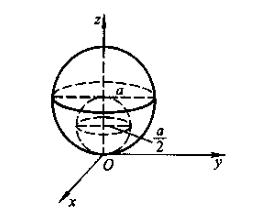
\includegraphics[width=4cm]{1.png}\\

\end{figure}
\newline
用球坐标换元,容易得$\theta$和$\varphi$的变化范围分别是$[0,\pi/2]$和$[0,2\pi]$.过坐标原点,在上半空间中作一条射线,这条射线将同两个球面相交,只要$\theta\neq\pi/2$, 交点就有两个,它们到原点的距离分别是$a\mathrm{cos}\ \theta$和$2a\mathrm{cos}\ \theta$,这就是说,对任意固定的$\theta \in [0,\pi/2]$,$r$的变化范围是$[a\mathrm{cos}\ \theta,2a\mathrm{cos}\ \theta]$.这样,新变量的取值范围就都确定了.

\section{\leftline{广义极坐标,广义球坐标换元}}
广义极坐标和广义球坐标的换元一般是用在椭圆和椭球区域上的,需要注意的是Jacobi行列式分别变为了$abr$和$abcr^{2}\mathrm{sin}\ \varphi$,需要注意在这个里面$r$的取值范围是$[0,1]$(这个也不是很难我就不多讲了)

\section{\leftline{不规则区域的换元}}

(1)计算$$\iint_{D}(x^{2}+y^{2})\mathrm{d}x\mathrm{d}y$$

其中$D$是由曲线$x^{2}-y^{2}=1,x^{2}-y^{2}=2,xy=1$和$xy=2$围成的图形在第一象限中的那部分.

(2)计算$$\iint_{D}\frac{3x}{y^{2}+xy^{3}}\mathrm{d}x\mathrm{d}y$$

其中$D$是由曲线$y^{2}=x,y^{2}=3x,xy=1$和$xy=3$围成的有界闭区域.

(3)计算$$\iint_{D}\frac{(\sqrt{x}+\sqrt{y})^{4}}{x^{2}}\mathrm{d}x\mathrm{d}y$$

其中$D$是由$x$轴,$y=x,\sqrt{x}+\sqrt{y}=1$和$\sqrt{x}+\sqrt{y}=2$围成的有界闭区域.
\newline
\newline
这种题一般都是令$u=f(x,y),v=g(x,y)$使得$u,v$的取值为矩形闭区域.但是对于某些题,求出用$x,y$来表示的$u,v$是困难的,所以这种换元的Jacobi行列式$\frac{\partial (x,y)}{\partial (u,v)}$也不易求出, 然而我们可以先求出$\frac{\partial (u,v)}{\partial (x,y)}$(这个非常好求,只需要将$u,v$看成自变量然后求$x,y$对$u,v$的偏导数即可),再利用两者为倒数关系(根据隐映射定理可以推出)求出所求的Jacobi行列式.
\section{\leftline{柱面,抛物面,锥面,球相交问题}}

有一大类题目的积分区域是柱面,抛物面,锥面,球等旋转体互相相交所截的部分,这些积分区域的特点是在z轴上的投影都是规则的,所以可以用柱坐标换元.
\newline
\newline
计算三重积分$$I=\iiint_{D}x^{2}\sqrt{x^{2}+y^{2}}\mathrm{d}x\mathrm{d}y\mathrm{d}z$$
其中$D$是曲面$z=x^{2}+y^{2}$和$z=\sqrt{x^{2}+y^{2}}$围成的部分.

\section{\leftline{利用对称性简化积分计算}}
(1)计算二重积分$$I=\iint_{D}(3x^{3}+x^{2}+y^{2}+2x-2y+1)\mathrm{d}x\mathrm{d}y$$
其中$D$=\{$(x,y)$:$1\leq x^{2}+(y-1)^{2}\leq2$,且$x^{2}+y^{2}\leq1$\}

(2)计算三重积分$$\iiint_{x^{2}+y^{2}+z^{2}\leq1}(x+y+z)^{2}\mathrm{d}x\mathrm{d}y\mathrm{d}z$$

\section{\leftline{正交变换}}

这种题吉大的教材挺重视的,但是其他高校的教材好像并不重视.


(1)常数$a,b$不全为0,求证:$$\iint_{x^{2}+y^{2}\leq1}f(ax+by+c)\mathrm{d}x\mathrm{d}y=2\int^{1}_{-1}\sqrt{1-t^{2}}f(t\sqrt{a^{2}+b^{2}}+c)\mathrm{d}t$$

\textbf{解题思路:}正交变换是指坐标轴旋转的变换,它的特点是坐标轴只旋转,坐标轴不伸缩,之间的夹角不变,所以对于一个圆心在原点的圆$x^{2}+y^{2}=r^{2}$来说,坐标轴旋转后的图形仍然是圆,并且位置仍然在圆心,半径不变.(想一想经过非正交变换后的圆可能会变成什么样的图案?)也就是说如果有正交变换$(u,v)^{\mathrm{T}}=A(x,y)^{\mathrm{T}}$,那么$x^{2}+y^{2}=r^{2}$变为$u^{2}+v^{2}=r^{2}$,仍然是圆(即新变量的积分区域也很容易确定)这就给计算提供了方便.

对于正交变换的Jacobi行列式,可以证明Jacobi行列式的值就等于相应的正交矩阵的行列式的值.而正交矩阵的行列式的值只有$\pm 1$,所以换元的时候就只需要把dx换成du,dy换成dv就可以了.

那么 如何来构造正交变换呢?对于上面的(1)来说,我们自然是希望$f$里面只有一个未知量,这样才能化为定积分.一个很自然的想法就是令$t=ax+by$(当然,换元$t=ax+by+c$可能更自然的会想到,但是正交变换中是不能带有常数的),但是我们还需要另外一个变元,不妨设$u=cx+dy$(之所以这样设是因为正交变换都是线性变换,不可能出现$u=cx^{2}+dy^{3}$等).所以求出对应的正交矩阵是
\begin{equation}\nonumber
{
\left( \begin{array}{ccc}
a& b &\\
c& d &
\end{array}
\right )}
\end{equation}

这个矩阵的两个行向量应该互相垂直,所以应有$c=-kb,d=ka$
并且两个行向量的模应该都为1(根据这个条件在前面乘上相应的系数),所以最后的正交变换矩阵是
\begin{equation}\nonumber
{
\left( \begin{array}{ccc}
\frac{a}{\sqrt{a^{2}+b^{2}}}& \frac{b}{\sqrt{a^{2}+b^{2}}} &\\
\frac{-b}{\sqrt{a^{2}+b^{2}}}& \frac{a}{\sqrt{a^{2}+b^{2}}} &
\end{array}
\right )}
\end{equation}

所以$t=\frac{a}{\sqrt{a^{2}+b^{2}}}x+\frac{b}{\sqrt{a^{2}+b^{2}}}y,u=\frac{-b}{\sqrt{a^{2}+b^{2}}}x+\frac{a}{\sqrt{a^{2}+b^{2}}}y,$就是正交变换.再根据正交变换圆的积分区域还是圆,dxdy=dtdu得到$$\iint_{x^{2}+y^{2}\leq1}f(ax+by)\mathrm{d}x\mathrm{d}y=\iint_{t^{2}+u^{2}\leq1}f(\sqrt{a^{2}+b^{2}}t)\mathrm{d}u\mathrm{d}t$$
注意到被积函数已经与u无关,所以可以轻松转化为定积分.

\textbf{我们发现在上面的推导中,我们完全不需要完全求出正交矩阵},(只需要知道这样的正交矩阵是存在的,不需要求出)需要做的只是把变换$t=ax+by$前面乘一个系数$1/\sqrt{a^{2}+b^{2}}$ 使得系数的平方和是1即可.然后就可以用正交变换来求解.

(1)常数$a,b,c$不全为0,求证:$$\iint_{x^{2}+y^{2}+z^{2}\leq1}f(ax+by+cz)\mathrm{d}x\mathrm{d}y\mathrm{d}z=\pi\int^{1}_{-1}(1-t^{2})f(t\sqrt{a^{2}+b^{2}+c^{2}})\mathrm{d}t$$

\section{\leftline{二重积分对参数求导问题}}

\noindent\textbf{例:}

设$f$是单变量函数,连续可导,令$$F(t)=\iint_{[0,t]^{2}}f(xy)\mathrm{d}x\mathrm{d}y$$证明:

(1)$$F'(t)=\frac{2}{t}\left(F(t)+\iint_{[0,t]^{2}}xyf'(xy)\mathrm{d}x\mathrm{d}y\right)$$

(2)$$F'(t)=\frac{2}{t}\int_{0}^{t^{2}}f(s)\mathrm{d}s$$

\textbf{解:}(1)作变换$x=tu,y=tv$,其Jacobi行列式为$t^{2}$,所以$$F(t)=\iint_{[0,1]^{2}}t^{2}f(t^{2}uv)\mathrm{d}u\mathrm{d}v$$
由于这时被积区域已不含$t$,所以直接对被积函数求导即可,有$$F'(t)=2t\iint_{[0,1]^{2}}f(t^{2}uv)\mathrm{d}u\mathrm{d}v+t^{2}\iint_{[0,1]^{2}}2tf'(t^{2}uv)\mathrm{d}u\mathrm{d}v$$
再用变换$u=x/t,v=y/t$换回到原来的变量$x,y$即可得证.

(2)

\begin{flalign}
F(t)&=\int_{0}^{t}\mathrm{d}x\int_{0}^{t}f(xy)\mathrm{d}y&\nonumber\\
&=\int_{0}^{t}\left(\int_{0}^{t}f(xy)\mathrm{d}y\right)\mathrm{d}x&\\
\end{flalign}
将$\int_{0}^{t}f(xy)\mathrm{d}y$,看成是关于x,y,t的函数$g(x,y,t)$,
\begin{flalign}
F'(t)&=\left(\int_{0}^{t}g(x,y,t)\mathrm{d}x\right)'&\\
&=g(t,y,t)+\int_{0}^{t}\frac{\partial g}{\partial t}(x,y,t)\mathrm{d}x&
\end{flalign}
由于$g$对$t$的导数为$f(tx)$,所以
\begin{flalign}
F'(t)&=\left(\int_{0}^{t}g(x,y,t)\mathrm{d}x\right)'&\\
&=\int_{0}^{t}f(ty)\mathrm{d}y+\int_{0}^{t}f(tx)\mathrm{d}x&
\end{flalign}
对两个积分分别作换元$s=ty,s=tx$,有
\begin{flalign}
F'(t)&=\frac{2}{t}\int_{0}^{t^{2}}f(s)\mathrm{d}s&
\end{flalign}
综上,(1)通过换元把积分区域的t转移到了被积函数中,使得积分区域是常数,这样就只需要对被积函数求导就可以了.(2)先变成累次积分再将内层的积分看成是关于x,y,t的函数,再利用含参变量积分中对参数的求导来计算.
\newline
\newline
模仿上面的例题,完成下面的练习

设$f$是单变量函数,连续可导,令$$F(t)=\iint_{[0,t]^{3}}f(xyz)\mathrm{d}x\mathrm{d}y\mathrm{d}z$$证明:

(1)$$F'(t)=\frac{3}{t}\left(F(t)+\iint_{[0,t]^{3}}xyzf'(xyz)\mathrm{d}x\mathrm{d}y\mathrm{d}z\right)$$

(2)$$F'(t)=\frac{3}{t}\int_{0}^{t^{3}}f(s)\mathrm{d}s$$

\newpage
\section{\leftline{答案}}
1.(1)$\pi (R^{2}\mathrm{e}^{R^{2}}-\mathrm{e}^{R^{2}}+1)$

1.(2)$\frac{2}{3}a^{3}(\frac{\pi}{2}-\frac{2}{3})$

1.(3)$\frac{5}{4}\pi a^{4}$

3.(1)$\frac{1}{2}$

3.(2)$\frac{2}{3}\mathrm{ln}\ 2$

3.(3)$\frac{15}{2}$

4.$\frac{\pi}{42}$

5.(1)$\frac{7\pi}{12}+\frac{7\sqrt{3}}{8}-2$

5.(2)$\frac{4\pi}{5}$
\end{document}
